\documentclass[11pt,a4paper]{article}

\usepackage[margin=1.5cm]{geometry}
\usepackage[T1]{fontenc}
\usepackage{lmodern}
\usepackage{amsmath,amssymb}
\usepackage{tikz}
\usepackage{graphicx}
\usepackage{caption}

% Load TikZ libraries
\usetikzlibrary{arrows.meta, positioning, fit, backgrounds, calc}

\begin{document}

% =============================================================================
% TITLE & OVERVIEW (Page 1)
% =============================================================================
\title{\textbf{\LARGE Audio-WAV-Synthesizer}\\[6pt]\large Software Architecture and UML Specifications}
\author{\textbf{Software Architecture Documentation}}
\date{\today}
\maketitle

\vspace{0.8cm}

\begin{abstract}
This document provides the formal software architectural design and object-oriented class specifications for the \textbf{Audio-WAV-Synthesizer} application. The system generates uncompressed 16-bit PCM WAV audio files from mathematical waveform models (Sine, Square, Sawtooth) modulated by a 4-stage piecewise linear ADSR (Attack, Decay, Sustain, Release) envelope.
\end{abstract}

\vspace{0.6cm}

\section*{Document Overview}
\begin{itemize}\setlength\itemsep{0.6em}
    \item \textbf{Section 1 (Page 2) -- UML Class Diagram:} Details the class hierarchy, inheritance trees, private/protected state representations, public interfaces, configuration containers, and binary serializer utilities with symmetrical center-aligned enumeration layout.
    \item \textbf{Section 2 (Page 3) -- System Architectural Diagram:} Outlines the three-tier decoupled system architecture encompassing the User Interface Layer (CLI and interactive FTXUI TUI), Core Synthesizer Engine (\texttt{synth\_core} library), and the Storage/Output Layer with clean, non-intersecting signal paths.
\end{itemize}

\clearpage

% =============================================================================
% 1. UML CLASS DIAGRAM (Page 2)
% =============================================================================
\section{UML Class Diagram}
The class structure decouples the abstract oscillator interface from concrete periodic waveforms, dynamic ADSR envelope gain calculations, and RIFF/WAVE file serialization.

\vspace{0.3cm}

\begin{center}
\resizebox{0.95\textwidth}{!}{%
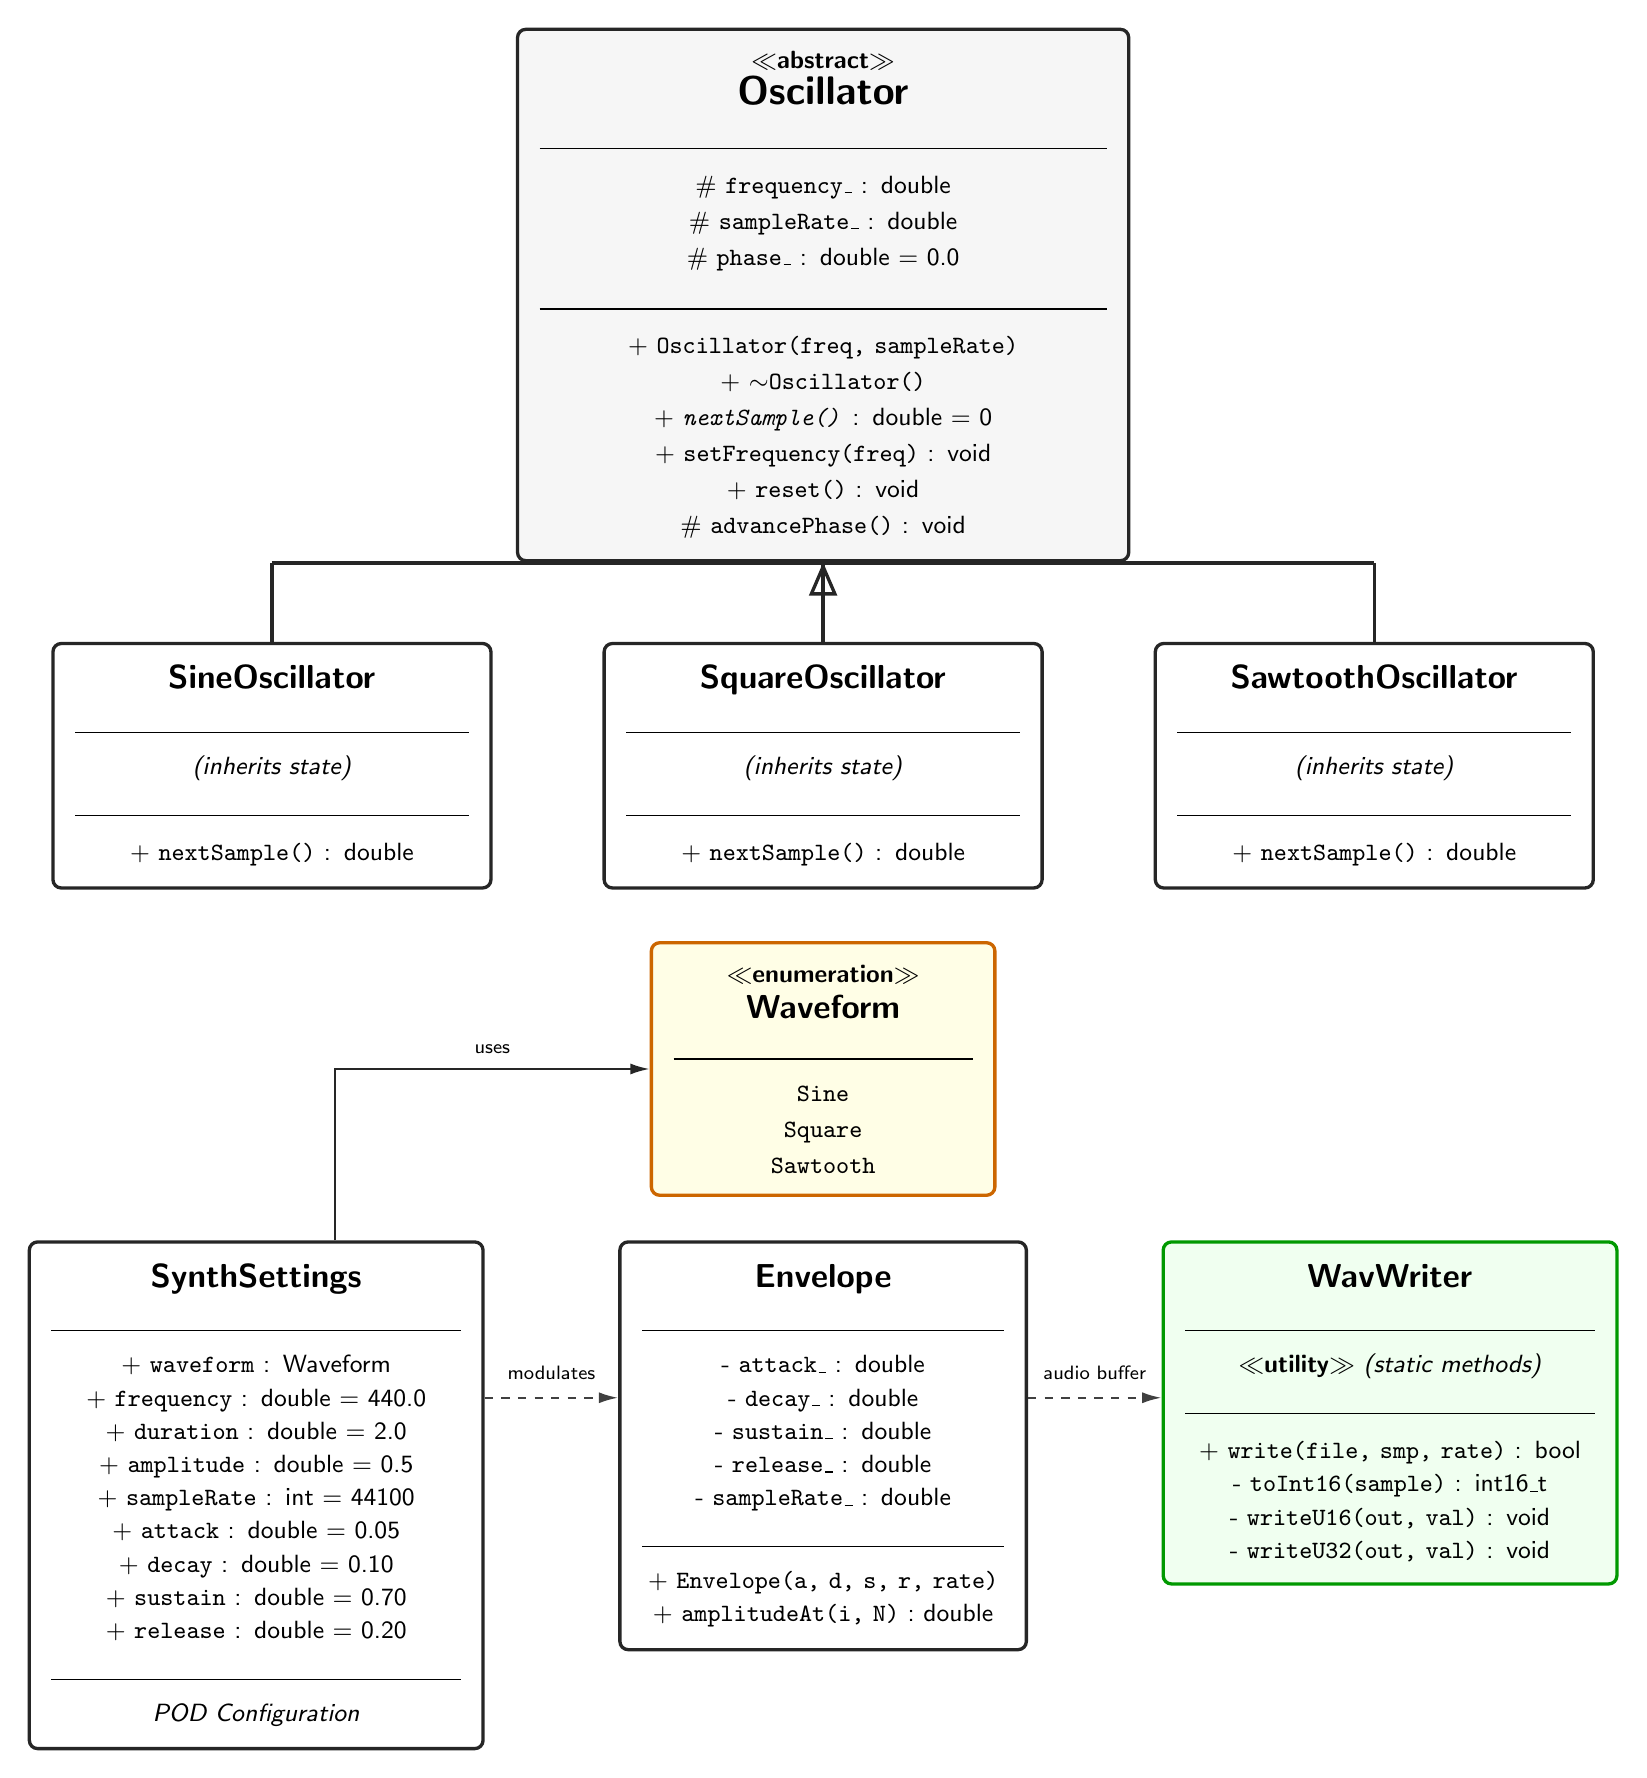
\begin{tikzpicture}[
    font=\small\sffamily,
    % Box styles with generous, clean padding
    umlClass/.style={
        draw=black!85,
        very thick,
        fill=white,
        rounded corners=3pt,
        inner sep=8pt,
        align=left
    },
    umlAbstract/.style={
        umlClass,
        fill=gray!7
    },
    umlEnum/.style={
        umlClass,
        fill=yellow!10,
        draw=orange!80!black
    },
    umlWriter/.style={
        umlClass,
        fill=green!6,
        draw=green!60!black
    },
    % Arrow styles
    depend/.style={
        -{Latex[length=7pt, width=4pt]},
        dashed,
        thick,
        draw=black!75
    },
    assoc/.style={
        -{Latex[length=7pt, width=4pt]},
        thick,
        draw=black!85
    }
]

    % =========================================================================
    % 1. TOP ROW: Abstract Base Class (Oscillator) - Anchor North at (0, 0)
    % =========================================================================
    \node[umlAbstract, text width=7.2cm, anchor=north] (oscillator) at (0, 0) {
        \centering $\ll$\textbf{abstract}$\gg$\\[2pt]
        \centering\textbf{\Large Oscillator}\\[5pt]
        \rule{\linewidth}{0.5pt}\\[5pt]
        \small
        \# \texttt{frequency\_} : double\\[2pt]
        \# \texttt{sampleRate\_} : double\\[2pt]
        \# \texttt{phase\_} : double = 0.0\\[5pt]
        \rule{\linewidth}{0.5pt}\\[5pt]
        \small
        + \texttt{Oscillator(freq, sampleRate)}\\[2pt]
        + \texttt{$\sim$Oscillator()}\\[2pt]
        + \texttt{\textit{nextSample()}} : double = 0\\[2pt]
        + \texttt{setFrequency(freq)} : void\\[2pt]
        + \texttt{reset()} : void\\[2pt]
        \# \texttt{advancePhase()} : void\\[3pt]
    };

    % =========================================================================
    % 2. INHERITANCE TREE (Standard UML Bus Bar with Open Triangle)
    % =========================================================================
    % Horizontal bus bar at y = -6.8, leaving clean clearance below Oscillator
    \coordinate (bus) at (0, -6.8);

    % Stem from bus bar up to Oscillator south with open triangle
    \draw[very thick, draw=black!85, -{Triangle[open, length=12pt, width=10pt]}] (bus) -- (oscillator.south);

    % Horizontal distribution bus bar
    \draw[very thick, draw=black!85] (-7.0, -6.8) -- (7.0, -6.8);

    % Vertical drop lines to each derived class (1.0 cm drop stem)
    \draw[very thick, draw=black!85] (-7.0, -6.8) -- (-7.0, -7.8);
    \draw[very thick, draw=black!85] (0, -6.8) -- (0, -7.8);
    \draw[very thick, draw=black!85] (7.0, -6.8) -- (7.0, -7.8);

    % =========================================================================
    % 3. SECOND ROW: Concrete Waveform Oscillators (Anchor North at y = -7.8)
    % =========================================================================
    % Wide text width (5.0cm) guarantees "+ nextSample() : double" fits on ONE line
    \node[umlClass, text width=5.0cm, anchor=north] (sineOsc) at (-7.0, -7.8) {
        \centering\textbf{\large SineOscillator}\\[5pt]
        \rule{\linewidth}{0.5pt}\\[4pt]
        \centering\textit{(inherits state)}\\[4pt]
        \rule{\linewidth}{0.5pt}\\[5pt]
        \small + \texttt{nextSample()} : double\\[2pt]
    };

    \node[umlClass, text width=5.0cm, anchor=north] (squareOsc) at (0, -7.8) {
        \centering\textbf{\large SquareOscillator}\\[5pt]
        \rule{\linewidth}{0.5pt}\\[4pt]
        \centering\textit{(inherits state)}\\[4pt]
        \rule{\linewidth}{0.5pt}\\[5pt]
        \small + \texttt{nextSample()} : double\\[2pt]
    };

    \node[umlClass, text width=5.0cm, anchor=north] (sawOsc) at (7.0, -7.8) {
        \centering\textbf{\large SawtoothOscillator}\\[5pt]
        \rule{\linewidth}{0.5pt}\\[4pt]
        \centering\textit{(inherits state)}\\[4pt]
        \rule{\linewidth}{0.5pt}\\[5pt]
        \small + \texttt{nextSample()} : double\\[2pt]
    };

    % =========================================================================
    % 4. THIRD ROW (MIDDLE TIER): Waveform Enumeration (Anchor North at y = -11.6)
    % =========================================================================
    % Sits with 1.4 cm clear gap below SquareOscillator and 1.4 cm clear gap above Envelope
    \node[umlEnum, text width=3.8cm, anchor=north] (waveformEnum) at (0, -11.6) {
        \centering $\ll$\textbf{enumeration}$\gg$\\[2pt]
        \centering\textbf{\large Waveform}\\[4pt]
        \rule{\linewidth}{0.5pt}\\[4pt]
        \centering\small
        \texttt{Sine}\\[2pt]
        \texttt{Square}\\[2pt]
        \texttt{Sawtooth}\\[2pt]
    };

    % =========================================================================
    % 5. FOURTH ROW (BOTTOM): SynthSettings, Envelope, and WavWriter (Anchor North at y = -15.4)
    % =========================================================================
    % Left: SynthSettings (centered at -7.2, text width=5.2cm prevents ANY attribute wrapping)
    \node[umlClass, text width=5.2cm, anchor=north] (settings) at (-7.2, -15.4) {
        \centering\textbf{\large SynthSettings}\\[5pt]
        \rule{\linewidth}{0.5pt}\\[4pt]
        \small
        + \texttt{waveform} : Waveform\\[1pt]
        + \texttt{frequency} : double = 440.0\\[1pt]
        + \texttt{duration} : double = 2.0\\[1pt]
        + \texttt{amplitude} : double = 0.5\\[1pt]
        + \texttt{sampleRate} : int = 44100\\[1pt]
        + \texttt{attack} : double = 0.05\\[1pt]
        + \texttt{decay} : double = 0.10\\[1pt]
        + \texttt{sustain} : double = 0.70\\[1pt]
        + \texttt{release} : double = 0.20\\[4pt]
        \rule{\linewidth}{0.5pt}\\[4pt]
        \centering\textit{POD Configuration}\\[2pt]
    };

    % Center: Envelope (centered at 0, text width=4.6cm fits constructors and methods on single lines)
    \node[umlClass, text width=4.6cm, anchor=north] (envelope) at (0, -15.4) {
        \centering\textbf{\large Envelope}\\[5pt]
        \rule{\linewidth}{0.5pt}\\[4pt]
        \small
        - \texttt{attack\_} : double\\[1pt]
        - \texttt{decay\_} : double\\[1pt]
        - \texttt{sustain\_} : double\\[1pt]
        - \texttt{release\_} : double\\[1pt]
        - \texttt{sampleRate\_} : double\\[4pt]
        \rule{\linewidth}{0.5pt}\\[4pt]
        \small
        + \texttt{Envelope(a, d, s, r, rate)}\\[1pt]
        + \texttt{amplitudeAt(i, N)} : double\\[2pt]
    };

    % Right: WavWriter (centered at +7.2, text width=5.2cm fits "+ write(file, smp, rate) : bool" on one line)
    \node[umlWriter, text width=5.2cm, anchor=north] (wavWriter) at (7.2, -15.4) {
        \centering\textbf{\large WavWriter}\\[5pt]
        \rule{\linewidth}{0.5pt}\\[4pt]
        \centering $\ll$\textbf{utility}$\gg$ \textit{(static methods)}\\[4pt]
        \rule{\linewidth}{0.5pt}\\[5pt]
        \small
        + \texttt{write(file, smp, rate)} : bool\\[1pt]
        - \texttt{toInt16(sample)} : int16\_t\\[1pt]
        - \texttt{writeU16(out, val)} : void\\[1pt]
        - \texttt{writeU32(out, val)} : void\\[2pt]
    };

    % =========================================================================
    % 6. ASSOCIATIONS & DEPENDENCIES (Generous 2.3 cm horizontal clearance)
    % =========================================================================
    % SynthSettings -> Waveform: Clean orthogonal route traveling exclusively in open space
    \draw[assoc] ([xshift=1.0cm]settings.north) |- node[near end, above=2pt, font=\scriptsize\sffamily] {uses} (waveformEnum.west);

    % SynthSettings -> Envelope: Clean horizontal line across 2.3 cm gap at y = -17.4
    \draw[depend] ([yshift=-2.0cm]settings.north east) -- node[midway, above=3pt, font=\scriptsize\sffamily] {modulates} ([yshift=-2.0cm]envelope.north west);

    % Envelope -> WavWriter: Clean horizontal line across 2.3 cm gap at y = -17.4
    \draw[depend] ([yshift=-2.0cm]envelope.north east) -- node[midway, above=3pt, font=\scriptsize\sffamily] {audio buffer} ([yshift=-2.0cm]wavWriter.north west);

\end{tikzpicture}
}
\captionof{figure}{UML Class Diagram for Audio-WAV-Synthesizer Core.}
\end{center}

\clearpage

% =============================================================================
% 2. SYSTEM ARCHITECTURAL DIAGRAM (Page 3)
% =============================================================================
\section{System Architectural Diagram}
The application follows a three-tier decoupled architecture separating presentation frontends, signal synthesis pipelines, and binary audio serialization.

\vspace{0.3cm}

\begin{center}
\resizebox{0.95\textwidth}{!}{%
\begin{tikzpicture}[
    font=\small\sffamily,
    % Box styling with balanced, clean padding
    box/.style={
        draw=black!85,
        thick,
        fill=white,
        rounded corners=3pt,
        align=center,
        inner sep=9pt
    },
    flowArrow/.style={
        -{Stealth[length=7pt, width=5pt]},
        very thick,
        draw=black!85
    }
]

    % =========================================================================
    % LAYER 1: USER INTERFACE LAYER (y = 0)
    % =========================================================================
    \node[box, fill=blue!8, text width=5.6cm] (cli) at (-4.0, 0) {
        \textbf{\large CLI Frontend (\texttt{synth})}\\[3pt]
        \scriptsize Parses CLI args (\texttt{--freq}, \texttt{--wave}, etc.),\\validates ranges, triggers audio rendering.
    };

    \node[box, fill=blue!8, text width=5.6cm] (tui) at (4.0, 0) {
        \textbf{\large Interactive TUI (\texttt{synth-tui})}\\[3pt]
        \scriptsize FTXUI interactive GUI with real-time waveform canvas,\\ADSR envelope graph, and parameter sliders.
    };

    \begin{scope}[on background layer]
        \node[fill=gray!8, draw=black!45, dashed, thick, rounded corners=6pt,
              fit=(cli) (tui), inner ysep=20pt, inner xsep=16pt] (layer1) {};
        % Title INSIDE the dotted box at top-left
        \node[anchor=north west, font=\bfseries\footnotesize, text=black!85]
              at ([xshift=10pt, yshift=-7pt]layer1.north west) {1. User Interface Layer (Executables)};
    \end{scope}

    % =========================================================================
    % LAYER 2: CORE SYNTHESIZER ENGINE (y = -5.0 to -8.6)
    % =========================================================================
    \node[box, fill=indigo!8, text width=5.6cm] (settings) at (-4.0, -5.0) {
        \textbf{\large Configuration / Settings}\\[3pt]
        \scriptsize \texttt{SynthSettings} struct \& \texttt{Waveform} enum\\Frequency, duration, sample rate, ADSR.
    };

    \node[box, fill=indigo!8, text width=5.6cm] (pipeline) at (4.0, -5.0) {
        \textbf{\large Rendering Pipeline (\texttt{render})}\\[3pt]
        \scriptsize Computes output audio sample buffer:\\[2pt]
        $\text{sample}[i] = \text{osc} \cdot \text{env} \cdot \text{amp}$
    };

    % DSP Core: Correct subsystem descriptions
    \node[box, fill=white, text width=12.4cm] (dspCore) at (0, -8.6) {
        \textbf{\large DSP Core Sound Generation Subsystems (\texttt{synth\_core})}\\[5pt]
        \begin{tabular}{p{5.6cm}@{\hspace{0.8cm}}p{5.6cm}}
            \centering\textbf{\normalsize Oscillator Hierarchy} & \centering\textbf{\normalsize ADSR Envelope Generator}\\[2pt]
            \centering\scriptsize Sine, Square, Sawtooth periodic generators & \centering\scriptsize 4-Stage piecewise linear modulator
        \end{tabular}
    };

    \begin{scope}[on background layer]
        \node[fill=blue!4, draw=blue!50!black, dashed, thick, rounded corners=6pt,
              fit=(settings) (pipeline) (dspCore), inner ysep=24pt, inner xsep=16pt] (layer2) {};
        % Title INSIDE the dotted box — two compact lines staying well clear of dataflow arrows
        \node[anchor=north west, font=\bfseries\footnotesize, text=black!85]
              at ([xshift=10pt, yshift=-7pt]layer2.north west) {\begin{tabular}{@{}l@{}}\textbf{2. Core Synthesizer Engine}\\\scriptsize\texttt{(synth\_core Static Library)}\end{tabular}};
    \end{scope}

    % =========================================================================
    % LAYER 3: STORAGE & FILE OUTPUT (y = -12.6)
    % =========================================================================
    \node[box, fill=green!8, text width=6.6cm] (wavWriter) at (-2.0, -12.6) {
        \textbf{\large WAV Serializer (\texttt{WavWriter})}\\[3pt]
        \scriptsize 16-bit PCM quantization, Little-Endian bit encoding,\\44-byte standard RIFF/WAVE header assembly.
    };

    \node[box, fill=green!18, text width=4.0cm] (wavFile) at (5.0, -12.6) {
        \textbf{\large Output File}\\[3pt]
        \scriptsize \texttt{tone.wav}\\(Standard 16-bit PCM)
    };

    \begin{scope}[on background layer]
        \node[fill=green!4, draw=green!60!black, dashed, thick, rounded corners=6pt,
              fit=(wavWriter) (wavFile), inner ysep=24pt, inner xsep=16pt] (layer3) {};
        % Title INSIDE the dotted box — two compact lines staying well clear of dataflow arrows
        \node[anchor=north west, font=\bfseries\footnotesize, text=black!85]
              at ([xshift=10pt, yshift=-7pt]layer3.north west) {\begin{tabular}{@{}l@{}}\textbf{3. Storage and Output Layer}\\\scriptsize\texttt{(RIFF/WAVE Audio File)}\end{tabular}};
    \end{scope}

    % =========================================================================
    % CLEAN DATAFLOW ARROWS (Zero overlap with text, boxes, or layer titles)
    % =========================================================================
    % UI Bus Bar: Clean horizontal bus in open space between Layer 1 and Layer 2 (at y = -2.2)
    \draw[very thick, draw=black!85] (cli.south) -- (-4.0, -2.2);
    \draw[very thick, draw=black!85] (tui.south) -- (4.0, -2.2);
    \draw[very thick, draw=black!85] (-4.0, -2.2) -- (4.0, -2.2);

    % Single clean arrow dropping from the bus bar into Configuration / Settings
    % Drops vertically at x = -1.6, which is > 1.6 cm clear to the right of Layer 2 title
    \draw[flowArrow] (-1.6, -2.2) -- (-1.6, -2.2 |- settings.north);

    % Settings -> Rendering Pipeline (straight horizontal across 2.4 cm gap)
    \draw[flowArrow] (settings.east) -- (pipeline.west);

    % Rendering Pipeline -> DSP Core (straight vertical drop at x = 4.0)
    \draw[flowArrow] (pipeline.south) -- (pipeline.south |- dspCore.north);

    % DSP Core -> WavWriter (clean straight vertical drop at x = -0.6)
    % Drops at x = -0.6, which is > 2.2 cm clear to the right of Layer 3 title
    % Label sits comfortably in the 2.4 cm vertical gap between Layer 2 and Layer 3
    \draw[flowArrow] ([xshift=-0.6cm]dspCore.south) -- node[midway, fill=white, inner sep=3pt, font=\scriptsize\sffamily] {Buffer: \texttt{std::vector<double>}} ([xshift=1.4cm]wavWriter.north);

    % WavWriter -> Output File (clean horizontal arrow with label neatly placed above)
    \draw[flowArrow] (wavWriter.east) -- node[midway, above=3pt, font=\scriptsize\sffamily] {Binary Stream} (wavFile.west);

\end{tikzpicture}
}
\captionof{figure}{Three-tier architectural diagram of the Audio-WAV-Synthesizer.}
\end{center}

\end{document}
